\section{Zielsetzung}
In diesem Versuch soll die Leerlaufspannung und der Innenwiderstand einer Spannungsquelle
bestimmt werden.

\section{Theorie}
Die Leerlaufspannung $U_0$ ist die Spannung an der Spannungsquelle, die über einen endlichen Zeitraum eine konstante
Leistung liefert, wo kein Strom $I$ fließt.
Mit einem Lastwiderstand $R_a$ fließt nun ein Strom $I$ und die Spannung, die man nun abgreifen kann,
nennt sich \enquote{Klemmspannung} $U_k$ und ist geringer als $U_0$.
In Abbildung (\ref{abb:1}) kann mit Hilfe der Maschenregel (zweites Kirschhoffsche Gesetz)
\begin{equation*}
  \sum_1 U_i = 0
\end{equation*}
und das Ohmische Gesetz
\begin{equation}
  U = R \cdot I
  \label{eq:1}
\end{equation}
die Formel für $U_0$ und $U_K$, mit Betrachtung der Stromrichtung darstellen.
\begin{equation}
  U_0= I (R_i + R_a) \,\, bzw. \,\, U_k=U_0 - I R_i
  \label{eq:2}
\end{equation}
\begin{figure}[H]
  \centering
  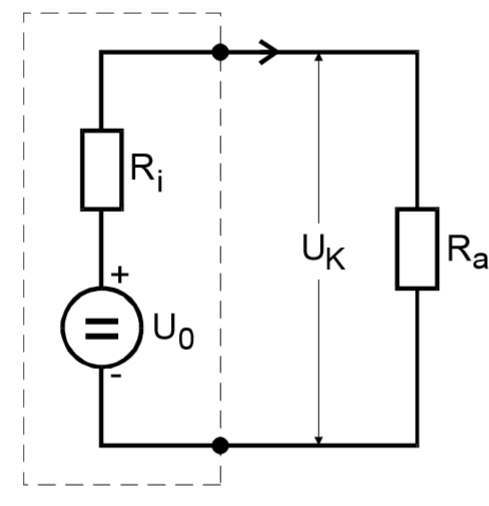
\includegraphics[width=10 cm, height= 7 cm]{Bild1.png}
  \caption{Stromkreis mit realen Spannungsquelle \cite{1}}
  \label{abb:1}
\end{figure}
Ebenso bescheibt in Abbildung(\ref{abb:1}) die geschrichelten Linien das Ersatzschaltbild dar
mit einer realen Spannungsquelle und einem Innenwiderstand $R_i$.
Aus Gleichung(\ref{eq:2}) folgt, dass für ein hochohmigen Widerstand $U_K \approx U_0$ gilt.\\
Durch den Innenwiderstand $R_i$  ist es nicht möglich aus einer idealen Spannungsquelle eine beliebig
hohe Leistung zu entnehmen. Die abgegebende Leistung kann an dem Lastwiderstand $R_a$ mit der Formel
\begin{equation}
  N(R_a) = I^2 \cdot R_a
  \label{eq:3}
\end{equation}
als Funktion dagestellt werden. Ist $R_a$ so gewählt, dass die Leistung $N$ einen Maximum annimmt, so nennt sich dies
eine Leistungsanpassung.
